\documentclass[a4,10pt]{aleph-notas}

%%--> Paquetes adicionales
\usepackage{enumitem}
\usepackage{textcomp}
\usepackage{subfig}
\usepackage{tikz}
\usepackage{pgfplots}
\usepackage{multicol}
\usetikzlibrary{matrix}
\pgfplotsset{compat=1.15}
\usetikzlibrary{cd}

%%--> Preámbulo del material
%% --> Paquetes comunes
\usepackage{listings}
\usepackage{enumitem}
\usepackage{lipsum}
\usepackage{booktabs}
\usepackage{todonotes}
\usepackage[spanish,onelanguage,vlined,linesnumbered]{algorithm2e}
\setuptodonotes{color=colordef!40, size=\footnotesize}
\newcommand{\porhacer}[1]{\todo[inline]{\textbf{Por hacer:} #1}}

%% --> Definición de colores
\definecolor{codegreen}{HTML}{A5BE00}
\definecolor{codegray}{rgb}{0.5,0.5,0.5}
\definecolor{codepurple}{rgb}{0.58,0,0.82}
\definecolor{backcolour}{rgb}{0.95,0.95,0.92}

%% --> Estilo para código
\lstdefinestyle{mystyle}{
    language={[LaTeX]TeX}, % lenguaje
    basicstyle=\bfseries\ttfamily,
    keywordstyle=\color{colordef},
    commentstyle=\color{codegreen},
    inputencoding=utf8,
    showstringspaces=false,
    flexiblecolumns=true,
    stringstyle=\ttfamily\color{blue},
    extendedchars=true,
    emph={rm,bf,it,sf}, %...
    literate=%
    {ó}{{\'o}}1%
    {í}{{\'i}}1%
    {á}{{\'a}}1%
    {ú}{{\'u}}1%
}

%% --> Selección de estilo para el código
\lstset{
    style=mystyle,escapeinside={(*@}{@*)}
}

% Blancos tipográficos
\newcommand{\mq}{\hspace{0.5em}}  %medio cuadratín
\newcommand{\tq}{\hspace{0.33em}} % un terio de cuadratín
\newcommand{\qq}{\hspace{0.25em}} % un cuarto de cuadratín
\newcommand{\fs}{\hspace{0.125em}} % un octavo de cuadratín
\newcommand{\ep}{\hspace{0.05em}} % espacio de pelo

%% --> Nota para el material
\newcommand{\informacion}{\noindent{\small\color{colordef}
El presente material fue desarrollado por:

\begin{center}
\textbf{Daniel Lara}\\
\emph{Facultad de Ciencias, Escuela Politécnica Nacional}\\[2mm]


\textbf{Andrés Merino}\\
\emph{Facultad de Ciencias Exactas y Naturales, Pontificia Universidad Católica del Ecuador}
\end{center}

\medskip\noindent
La versión actual del material es 1.3-(Noviembre 2021). En caso de encontrar inconsistencias o errores en el presente material se pueden comunicar a \href{mailto:daniel.lara@alephsub0.org}{daniel.lara@alephsub0.org}. Para más información puedes visitar nuestro sitio web: \href{https://alephsub0.org}{alephsub0.org}. Si deseas colaborar con el desarrollo de este material, el código fuente está disponible en:   
\url{https://github.com/alephsub0/LaTeX_Guias.git}. Cualquier aporte (\emph{Pull request}) será de gran ayuda para mejorar este material. 

\medskip\noindent

\includegraphics[height=10pt]{Imagenes/CreativeCommos/cc.xlarge.png}

\includegraphics[height=10pt]{Imagenes/CreativeCommos/by.xlarge.png}

\includegraphics[height=10pt]{Imagenes/CreativeCommos/nc.xlarge.png}
Esta obra se encuentra bajo licencia Atribución-NoComercial-CompartirIgual 4.0 Internacional (CC BY-NC-SA 4.0) Para más información puede visitar: \url{https://creativecommons.org/licenses/by-nc-sa/4.0/}


%% -- > Aquí se incluyen los nombres de los colaboradores de estas guías:
% \medskip\noindent
% Otros colaboradores: Katheryn Yánes
}}

%%--> Formato para títulos
\titleformat{name=\section,numberless}[display]
  {\vspace*{-2mm}\bfseries\scshape\centering}
    {}{1ex}
    {\color{colortext}\large\titlerule\vspace{.05ex}
     }
    [\color{colortext}\vspace{.2ex}\titlerule]

\titleformat{\subsubsection}
    {\color{colortext}\normalsize\bfseries}
    {\thesubsubsection}{1em}{}
    
%% --> Datos de las guias
\universidad{Curso de \LaTeX}
\autor{Proyecto Alephsub0}
\materia{Introducción a \LaTeX}

%% --> Logos de las guias
\logouno[4.5cm]{Imagenes/Logos/LogoAlephsub0-02.png}
\longtitulo{0.6\linewidth}
\fecha{Noviembre de 2021}

%% --> Nuevos ambientes
% \definecolor{coloryt}{rgb}{0.769,0.188,0.169}
%% Ambientes
\makeatletter
%%  Keys temporales: |colorlat|
\def\tcb@@colorlat{colordef!50!black}
    \tcbset{ colorlat/.code = {\def\tcb@@colorlat{#1} } }
%%  Estilo de YouTube
\tcbset{ postitbeta/.style ={
    % -> Opciones generales
    breakable,enhanced,
    before skip=2mm,after skip=3mm,
    colback=\tcb@@color!50,colframe=\tcb@@color!20!black,
    boxrule=0.4pt,
    drop fuzzy shadow,
    left=6mm,right=2mm,top=0.5mm,bottom=0.5mm,
    sharp corners,rounded corners=southeast,arc is angular,arc=3mm,
    parbox=false,
    underlay unbroken and last = {%
        \path[fill=tcbcolback!80!black]
        ([yshift=3mm]interior.south east) --++ (-0.4,-0.1) --++ (0.1,-0.2);
        \path[draw=tcbcolframe,shorten <=-0.05mm,shorten >=-0.05mm]
        ([yshift=3mm]interior.south east) --++ (-0.4,-0.1) --++ (0.1,-0.2);
        \path[fill=\tcb@@colorlat,draw=none]
        (interior.south west) rectangle node[white]{\tcb@@icono} ([xshift=5.5mm]interior.north west);
        },
    underlay = {%
        \path[fill=\tcb@@colorlat,draw=none]
        (interior.south west) rectangle node[white]{\tcb@@icono} ([xshift=5.5mm]interior.north west);
        }
    }
    }
\makeatother

%% Recuadro para enlaces de YouTube
\definecolor{coloryt}{HTML}{ffcccc}
\newtcolorbox{tcbyoutube}
    {icono=\faYoutubePlay,color=coloryt,colorlat=red,postitbeta,colframe=red,leftright skip=1cm}
    
%% Comando para enlaces de YouTube
\newcommand{\YouTube}[4]%
    {
        \begin{tcbyoutube}
            \parbox{0.30\linewidth}{\href{#2}{\includegraphics[width=\linewidth]{#3}}}
            \hspace{2mm}
            \parbox{0.65\linewidth}{\footnotesize
            \textbf{#1}\\[1mm]
            \faLink\ \url{#2}\\[2mm]
            \scriptsize
            #4}
        \end{tcbyoutube}
    }
    
%% Recuadro para enlaces
\definecolor{coloren}{HTML}{B9F2BC}
\newtcolorbox{tcbenlace}
    {icono=\faLink,color=coloren,postit,leftright skip=1cm,fontupper=\small}

%% Recuadro para impresión
\definecolor{colorimp}{HTML}{F8F8FF}
\newtcolorbox{tcbimprimir}
    {icono=\faPrint,color=colorimp,postit,leftright skip=1cm,fontupper=\small}

%% Ambiente para código
\definecolor{colcod}{RGB}{174,218,255}
\newtcolorbox{tcbcodigo}
    {icono=\faCode,color=colcod,postit,top=-2mm,bottom=-2mm,leftright skip=1cm,fontupper=\small}

%% Ambiente para código LaTeX  
\usepackage{minted}
\usemintedstyle{borland}
\tcbuselibrary{minted}
\tcbset{listing engine=minted}
\newtcblisting{tcbLaTeX}{%
    icono=\faCode,color=colcod,postit,top=0mm,bottom=0mm,
    leftright skip=1cm,fontupper=\small,
    minted language=latex,minted style=colorful,
    listing only}
% \newtcolorbox{tcbcodigo}
%     {icono=\faCode,color=colcod,postit,top=-2mm,bottom=-2mm,leftright skip=1cm,fontupper=\small}

%% Ambiente para figuras 
\newtcolorbox[blend into=figures]{figura}[2][]
    {float=h,capture=hbox,title={#2},every float=\centering,
    arc=0mm,left=2mm,right=2mm,
    boxrule=0pt,
    colback=colordef!10,
    colbacktitle=colordef!80,fonttitle=\small,
    enhanced,attach boxed title to bottom,center title,
    #1}

%% Ambiente para tablas 
\newtcolorbox[blend into=tables]{tabla}[2][]
    {float=h,capture=hbox,title={#2},every float=\centering,
    arc=0mm,left=2mm,right=2mm,
    boxrule=0pt,
    colback=colordef!10,
    colbacktitle=colordef!80,fonttitle=\small,
    enhanced,center title,
    #1}

%% Ambiente para código LaTeX desplegado
\newtcblisting{tcbLaTeXb}{%
    icono=\faCode,color=colcod,postit,top=0mm,bottom=0mm,
    fontupper=\small,
    minted language=latex,minted style=colorful,listing side text}
\newtcblisting{tcbLaTeXs}{%
    icono=\faCode,color=colcod,postit,top=0mm,bottom=0mm,
    fontupper=\small,
    minted language=latex,minted style=colorful}

%% Recuadro para comando en línea
\DeclareTotalTCBox{\miverb}{ v }{
    fontupper=\ttfamily,nobeforeafter,tcbox raise base,arc=0pt,outer arc=0pt,
    top=0pt,bottom=0pt,left=0mm,right=0mm,
    leftrule=0pt,rightrule=0pt,toprule=0.3mm,bottomrule=0.3mm,boxsep=0.5mm,
    colback=colcod!10!white,colframe=colcod!50!black}{#1}


% -- Datos del libro
\nota{Guía 5}
\tema{Tikz}

% \tikzset{
% every picture/.append style={
%   execute at begin picture={\deactivatequoting},
%   execute at end picture={\activatequoting}
%   }
% }

\begin{document}

\shorthandoff{<}
\shorthandoff{>}
\shorthandoff{"}

\encabezado

\informacion

\tableofcontents

\section{Tikz}

En esta sección estudiaremos la generación de gráficos mediante código, para este propósito tenemos dos opciones: PSTricks y TikZ; debido a la estructura de \LaTeX{} PSTricks está limitado únicamente a ser compatible con el compilador \TeX{} por este motivo vamos a escoger TikZ como el lenguaje para realizar nuestros gráficos. Para comenzar esta sección debemos incluir el paquete y sus opciones en el preámbulo de nuestro documento:

\begin{lstlisting}[frame=single]
\usepackage{tikz}
\pgfplotsset{compat=1.15}
\usepackage{pgfplots}
\end{lstlisting}


Una de las funcionalidades más prácticas de TikZ está en su capacidad de crear pequeños gráficos en medio del texto escrito. Por ejemplo, si se desea generar un pequeño círculo rojo en medio de este texto podemos usar el siguiente código:

\begin{lstlisting}[frame=single]
Este código nos muestra como crear un círculo -> \tikz \fill[orange] (1ex,1ex) circle (1ex);
\end{lstlisting}

\begin{center}
{ \fboxsep 12pt
\fcolorbox {black}{white}{
\begin{minipage}[t]{10cm}
Este código nos muestra como crear un círculo -> \tikz \fill[orange] (1ex,1ex) circle (1ex);
\end{minipage}
} }
\end{center}

Sin embargo, en la mayoría de los casos requerimos que se use el ambiente para la elaboración de gráficos más complejos. Para comenzar con la elaboración de gráficos, consideremos los comandos básicos para la generación de los mismos. 

\subsection{Comando \texttt{draw}}

Este comando es el más sencillo y nos permite trazar una linea entre los dos puntos: un ejemplo lo podemos ver a continuación

\begin{lstlisting}[frame=single]
\begin{tikzpicture}
    \draw (0,0) -- (2,2); % segmento
\end{tikzpicture}
\end{lstlisting}

\begin{center}
\begin{tikzpicture}
    \draw (0,0) -- (2,2); % segmento
    \end{tikzpicture}
\end{center}

Para una ayuda visual al momento de realizar nuestros gráficos, podemos recurrir a la opción \verb@[help lines]@ del comando \verb@\draw@, de esta manera tenemos el siguiente ejemplo:

\begin{lstlisting}[frame=single]
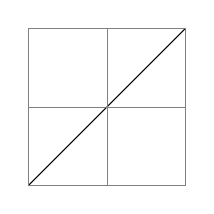
\begin{tikzpicture}
    \draw(0,0) -- (2,2); % segmento
    \draw[help lines] (0,0) grid (2,2);
\end{tikzpicture}
\end{lstlisting}

\begin{center}
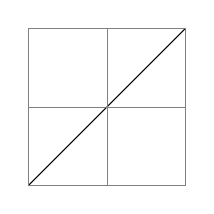
\begin{tikzpicture}
\draw (0,0) -- (2,2); % segmento
\draw[help lines] (0,0) grid (2,2);
\end{tikzpicture}
\end{center}

Una vez realizado nuestro gráfico, es importante poder manipular las dimensiones del mismo; para escalar un gráfico realizado en TikZ, recurrimos a la opción \verb@scale@ del ambiente, por ejemplo:

\begin{lstlisting}[frame=single]
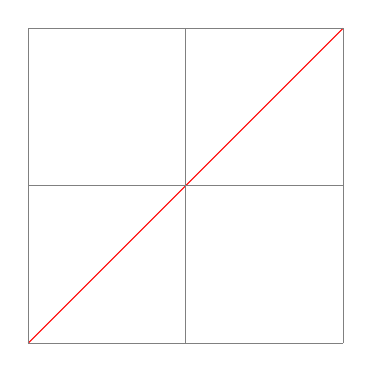
\begin{tikzpicture}[scale=2]
    \draw[red] (0,0) -- (2,2); % segmento
    \draw[help lines] (0,0) grid (2,2);
\end{tikzpicture}
\end{lstlisting}

\begin{center}
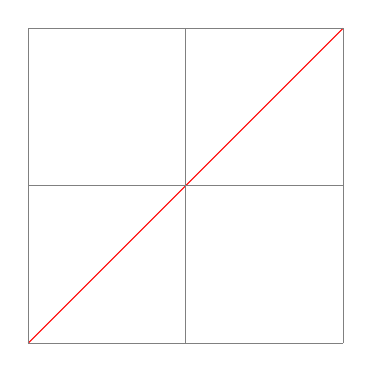
\begin{tikzpicture}[scale=2]
\draw[red] (0,0) -- (2,2); % segmento
\draw[help lines] (0,0) grid (2,2);
\end{tikzpicture}
\end{center}

Para escalar el gráfico con diferentes razones en cada eje usamos \verb@xscale@ y \verb@yscale@

\begin{lstlisting}[frame=single]
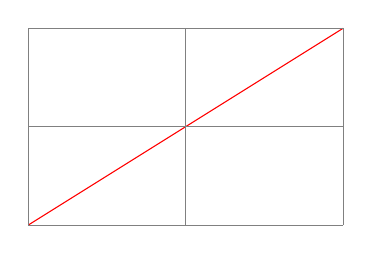
\begin{tikzpicture}[xscale=2,yscale=1.25]
    \draw[red] (0,0) -- (2,2); % segmento
    \draw[help lines] (0,0) grid (2,2);
\end{tikzpicture}
\end{lstlisting}

\begin{center}
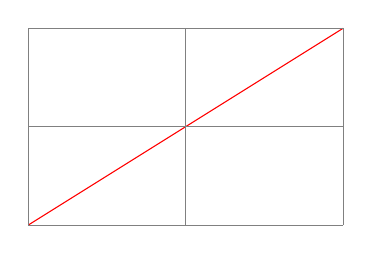
\begin{tikzpicture}[xscale=2,yscale=1.25]
    \draw[red] (0,0) -- (2,2); % segmento
    \draw[help lines] (0,0) grid (2,2);
\end{tikzpicture}
\end{center}

\subsubsection{Flechas}

En esta subsección aprenderemos a incluir «flechas» a las lineas que aprendimos a dibujar, estas se incluyen como argumentos del comando \verb@draw@ de la siguiente manera:

\begin{lstlisting}[frame=single]
\begin{tikzpicture}
    \draw [->] (0,0) -- (2,0);
    \draw [<-] (0, -0.5) -- (2,-0.5);
    \draw [|->] (0,-1) -- (2,-1);
\end{tikzpicture}
\end{lstlisting}

\begin{center}



\begin{tikzpicture}
    \draw [->] (0,0) -- (2,0);
    \draw [<-] (0, -0.5) -- (2,-0.5);
    \draw [|->] (0,-1) -- (2,-1);
\end{tikzpicture}
\end{center}

\begin{advertencia}
Las opciones \verb@|->@  y \verb@->@ tienen un conflicto con el paquete \verb@babel@ al momento de usar el idioma español, por ese motivo es necesario incluir las siguientes instrucciones luego del \verb@\begin{document}@:


\begin{verbatim}
\shorthandoff{<}
\shorthandoff{>}
\end{verbatim}

\end{advertencia}

\subsubsection{Grosor del trazo}

Para la modificación del grosor del trazo tenemos los siguientes ejemplos:

\begin{lstlisting}[frame=single]

\begin{tikzpicture}
    \draw [ultra thick] (0,1) -- (2,1);
    \draw [thick] (0,0.5) -- (2,0.5);
    \draw [thin] (0,0) -- (2,0);
\end{tikzpicture}
\end{lstlisting}

\begin{center}

\begin{tikzpicture}
\draw [ultra thick] (0,1) -- (2,1);
\draw [thick] (0,0.5) -- (2,0.5);
\draw [thin] (0,0) -- (2,0);
\end{tikzpicture}
\end{center}

Sin embargo, también es posible usar medidas personalizadas usando las unidades vistas en la primera guía; un ejemplo de 
ello se encuentra a continuación:

\begin{lstlisting}[frame=single]

\begin{tikzpicture}
    \draw [line width=12pt] (0,0) -- (2,0);
    \draw [line width=0.2cm] (4,.75) -- (5,.25);
\end{tikzpicture}
\end{lstlisting}

\begin{center}

\begin{tikzpicture}
\draw [line width=12pt] (0,0) -- (2,0);
\draw [line width=0.2cm] (4,.75) -- (5,.25);
\end{tikzpicture}
\end{center}

Por defecto, la unidad usada en TikZ es el punto tipográfico.

\subsubsection{Guiones y puntos}

\begin{lstlisting}[frame=single]
\begin{tikzpicture}
    \draw [dashed, ultra thick] (0,1) -- (2,1);
    \draw [dashed] (0, 0.5) -- (2,0.5);
    \draw [dotted] (0,0) -- (2,0);
\end{tikzpicture}
\end{lstlisting}

\begin{center}
\begin{tikzpicture}
    \draw [dashed, ultra thick] (0,1) -- (2,1);
    \draw [dashed] (0, 0.5) -- (2,0.5);
    \draw [dotted] (0,0) -- (2,0);
\end{tikzpicture}
\end{center}

\subsubsection{Colores}

\begin{lstlisting}[frame=single]
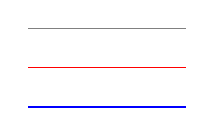
\begin{tikzpicture}
    \draw [gray] (0,1) -- (2,1);
    \draw [red] (0, 0.5) -- (2,0.5);
    \draw [blue] (0,0) -- (2,0);
\end{tikzpicture}
\end{lstlisting}

\begin{center}
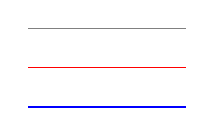
\begin{tikzpicture}
    \draw [gray] (0,1) -- (2,1);
    \draw [red] (0, 0.5) -- (2,0.5);
    \draw [blue] (0,0) -- (2,0);
\end{tikzpicture}
\end{center}

\subsubsection{Figuras geométricas}

\begin{lstlisting}[frame=single]
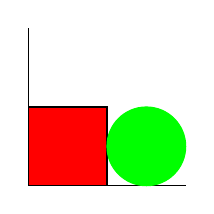
\begin{tikzpicture} % ejes
    \draw[thin] (0,2) -- (0,0) -- (2,0);
    % rectangulo borde negro, relleno rojo, esquina (0,0)
    \draw[black, fill=red] (0,0) rectangle(1,1);
    % circulo verde, centro =(1.5,.5) y radio 0.5cm
    \draw[green, fill=green] (1.5,0.5) circle [radius
    =0.5];
\end{tikzpicture}
\end{lstlisting}

\begin{center}
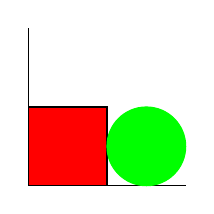
\begin{tikzpicture} % ejes
\draw[thin] (0,2) -- (0,0) -- (2,0);
% rectángulo borde negro, relleno rojo, esquina (0,0)
\draw[black, fill=red] (0,0) rectangle(1,1);
% círculo verde, centro =(1.5,.5) y radio 0.5cm
\draw[green, fill=green] (1.5,0.5) circle [radius
=0.5];
\end{tikzpicture}
\end{center}

\subsubsection{Más ejemplos}

\begin{lstlisting}[frame=single]
\begin{tikzpicture} % ejes
    \draw[thin, blue] (0,2) -- (0,0) -- (2,0);
    % segmento
    \draw[line width =0.051cm, red, dashed]
    (-1,-1) -- (1.5,1.5);
\end{tikzpicture}
\end{lstlisting}

\begin{center}
\begin{tikzpicture} % ejes
    \draw[thin, blue] (0,2) -- (0,0) -- (2,0);
    % segmento
    \draw[line width =0.051cm, red, dashed]
    (-1,-1) -- (1.5,1.5);
\end{tikzpicture}
\end{center}

\subsection{Curvas}

\begin{lstlisting}[frame=single]

\begin{tikzpicture}
    \draw [blue] (0,0) rectangle (1.5,1);
    \draw [red, ultra thick] (3,0.5) circle [radius=0.5];;
    \draw [gray] (6,0) arc [radius=1, start angle=45, end angle= 120];
\end{tikzpicture}
\end{lstlisting}

\begin{center}

\begin{tikzpicture}
\draw [blue] (0,0) rectangle (1.5,1);
\draw [red, ultra thick] (3,0.5) circle [radius=0.5];;
\draw [gray] (6,0) arc [radius=1, start angle=45, end angle= 120];
\end{tikzpicture}
\end{center}

\begin{lstlisting}[frame=single]
\begin{tikzpicture}
    \draw [<->, rounded corners, thick, purple] (0,2) -- (0,0) -- (3,0);
\end{tikzpicture}
\end{lstlisting}

\begin{center}
\begin{tikzpicture}
\draw [<->, rounded corners, thick, purple] (0,2) -- (0,0) -- (3,0);
\end{tikzpicture}
\end{center}

\subsection{Graficar funciones}

\begin{lstlisting}[frame=single]
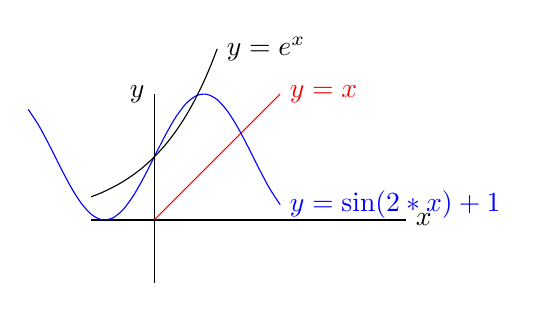
\begin{tikzpicture}[scale=0.8] % Escalamiento de la figura 80%
    \draw (-1,0) -- (4,0) node[right] {$x$}; % Ejes
    \draw (0,-1) -- (0, 2) node[left] {$y$};
    % Dominio: domain = a:b
    \draw[smooth, domain = 0:2, color=red] plot (\x,\x)node[right] {$y = x$
    };
    %\x r indica que x se mide en radianes
    \draw[smooth, domain = -2:2, color=blue] plot (\x,{sin(2*\x r)+1})
    node[right] {$y = \sin(2*x)+1$};
    \draw[smooth, domain = -1:1, color=black] plot (\x,{exp(\x)}) node[right
    ] {$y = e^x$};
\end{tikzpicture}
\end{lstlisting}

\begin{center}
    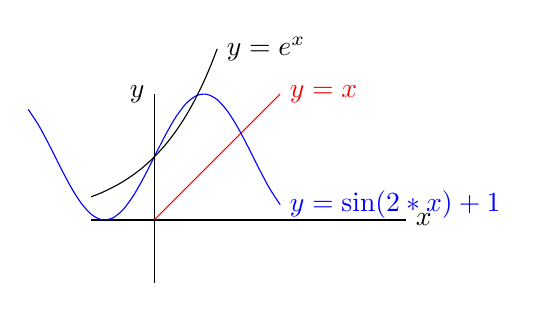
\begin{tikzpicture}[scale=0.8] % Escalamiento de la figura 80%
\draw (-1,0) -- (4,0) node[right] {$x$}; % Ejes
\draw (0,-1) -- (0, 2) node[left] {$y$};
% Dominio: domain = a:b
\draw[smooth, domain = 0:2, color=red] plot (\x,\x)node[right] {$y = x$
};
%\x r indica que x se mide en radianes
\draw[smooth, domain = -2:2, color=blue] plot (\x,{sin(2*\x r)+1})
node[right] {$y = \sin(2*x)+1$};
\draw[smooth, domain = -1:1, color=black] plot (\x,{exp(\x)}) node[right
] {$y = e^x$};
\end{tikzpicture}
\end{center}

\begin{lstlisting}[frame=single]
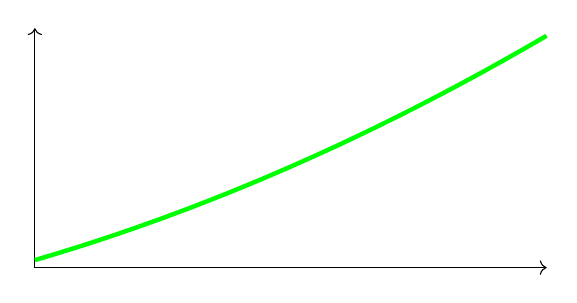
\begin{tikzpicture}[xscale=13,yscale=3.8]
    \draw [<->] (0,0.8) -- (0,0) -- (0.5,0);
    \draw[green, ultra thick, domain=0:0.5] plot (\x, {0.025+\x+\x*\x});
\end{tikzpicture}
\end{lstlisting}

\begin{center}
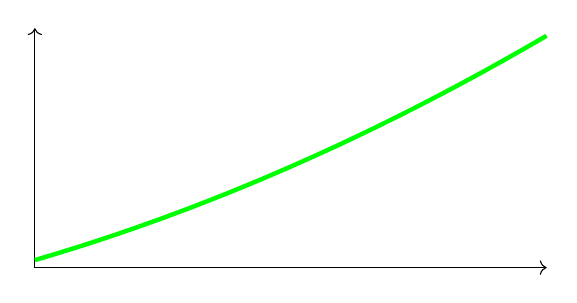
\begin{tikzpicture}[xscale=13,yscale=3.8]
\draw [<->] (0,0.8) -- (0,0) -- (0.5,0);
\draw[green, ultra thick, domain=0:0.5] plot (\x, {0.025+\x+\x*\x});
\end{tikzpicture}
\end{center}

\begin{lstlisting}[frame=single]
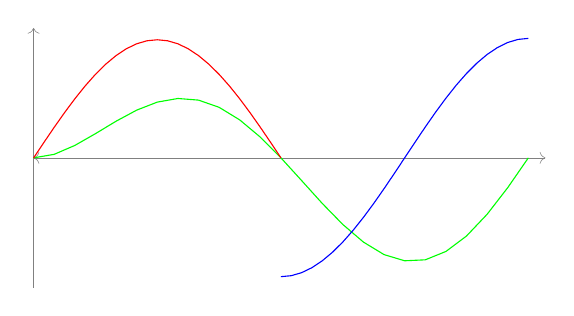
\begin{tikzpicture}[yscale=1.5]
    \draw [help lines, <->] (0,0) -- (6.5,0);
    \draw [help lines, ->] (0,-1.1) -- (0,1.1);
    \draw [green,domain=0:2*pi] plot (\x, {(sin(\x r)* ln(\x+1))/2});
    \draw [red,domain=0:pi] plot (\x, {sin(\x r)});
    \draw [blue, domain=pi:2*pi] plot (\x, {cos(\x r)*exp(\x/exp(2*pi))});
\end{tikzpicture}
\end{lstlisting}

\begin{center}
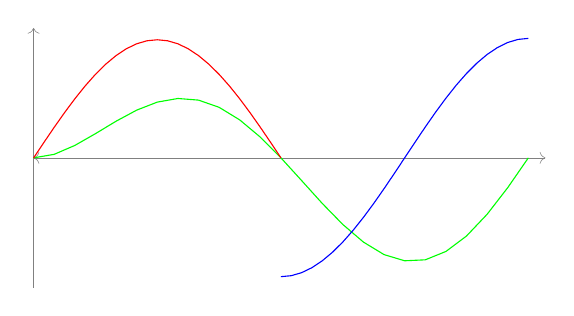
\begin{tikzpicture}[yscale=1.5]
\draw [help lines, <->] (0,0) -- (6.5,0);
\draw [help lines, ->] (0,-1.1) -- (0,1.1);
\draw [green,domain=0:2*pi] plot (\x, {(sin(\x r)* ln(\x+1))/2});
\draw [red,domain=0:pi] plot (\x, {sin(\x r)});
\draw [blue, domain=pi:2*pi] plot (\x, {cos(\x r)*exp(\x/exp(2*pi))});
\end{tikzpicture}
\end{center}

\subsection{Rellenos}

\begin{lstlisting}[frame=single]
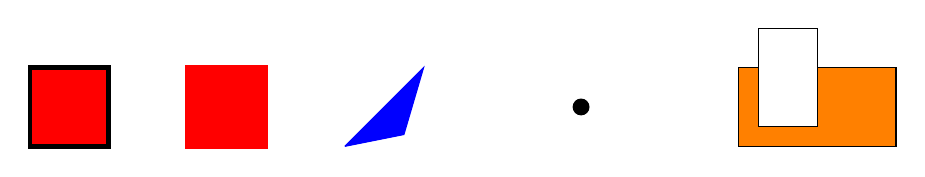
\begin{tikzpicture}
    \draw [fill=red,ultra thick] (0,0) rectangle (1,1);
    \draw [fill=red,ultra thick,red] (2,0) rectangle (3,1);
    \draw [blue, fill=blue] (4,0) -- (5,1) -- (4.75,0.15) -- (4,0);
    \draw [fill] (7,0.5) circle [radius=0.1];
    \draw [fill=orange] (9,0) rectangle (11,1);
    \draw [fill=white] (9.25,0.25) rectangle (10,1.5);
\end{tikzpicture}
\end{lstlisting}

\begin{center}
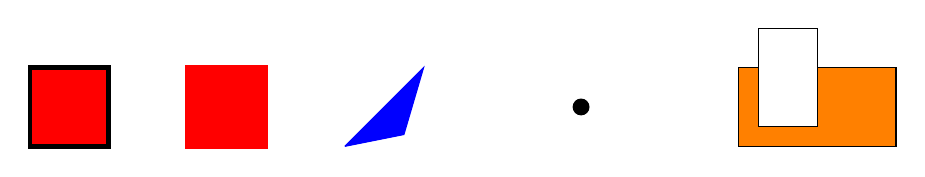
\begin{tikzpicture}
\draw [fill=red,ultra thick] (0,0) rectangle (1,1);
\draw [fill=red,ultra thick,red] (2,0) rectangle (3,1);
\draw [blue, fill=blue] (4,0) -- (5,1) -- (4.75,0.15) -- (4,0);
\draw [fill] (7,0.5) circle [radius=0.1];
\draw [fill=orange] (9,0) rectangle (11,1);
\draw [fill=white] (9.25,0.25) rectangle (10,1.5);
\end{tikzpicture}
\end{center}

\subsection{Etiquetas}

En esta sección vamos a aprender a incluir etiquetas en nuestros gráficos, para ello consideremos los siguientes ejemplos:

\begin{lstlisting}[frame=single]
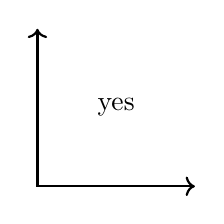
\begin{tikzpicture}
    \draw [thick, <->] (0,2) -- (0,0) -- (2,0);
    \node at (1,1) {yes};
\end{tikzpicture}
\end{lstlisting}

\begin{center}
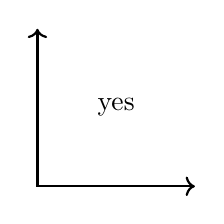
\begin{tikzpicture}
\draw [thick, <->] (0,2) -- (0,0) -- (2,0);
\node at (1,1) {yes};
\end{tikzpicture}
\end{center}

\begin{lstlisting}[frame=single]
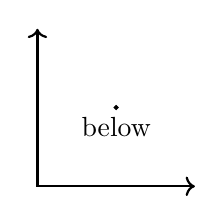
\begin{tikzpicture}
    \draw [thick, <->] (0,2) -- (0,0) -- (2,0);
    \draw[fill] (1,1) circle [radius=0.025];
    \node [below] at (1,1) {below};
\end{tikzpicture}
\end{lstlisting}

\begin{center}
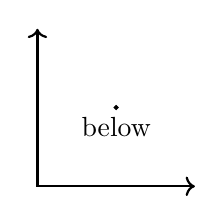
\begin{tikzpicture}
\draw [thick, <->] (0,2) -- (0,0) -- (2,0);
\draw[fill] (1,1) circle [radius=0.025];
\node [below] at (1,1) {below};
\end{tikzpicture}
\end{center}

\begin{lstlisting}[frame=single]
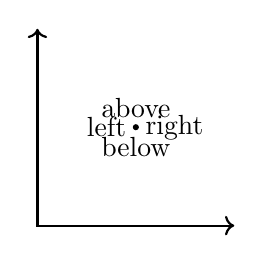
\begin{tikzpicture}[scale=1.25]
    \draw [thick, <->] (0,2) -- (0,0) -- (2,0);
    \draw[fill] (1,1) circle [radius=0.025];
    \node [below] at (1,1) {below};
    \node [above] at (1,1) {above};
    \node [left] at (1,1) {left};
    \node [right] at (1,1) {right};
\end{tikzpicture}
\end{lstlisting}

\begin{center}
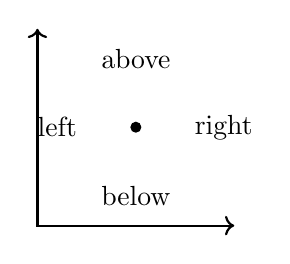
\begin{tikzpicture}[scale=1.25]
\draw [thick, <->] (0,2) -- (0,0) -- (2,0);
\draw[fill] (1,1) circle [radius=0.05];
\node [below] at (1,0.5) {below};
\node [above] at (1,1.5) {above};
\node [left] at (0.5,1) {left};
\node [right] at (1.5,1) {right};
\end{tikzpicture}
\end{center}

\begin{lstlisting}[frame=single]
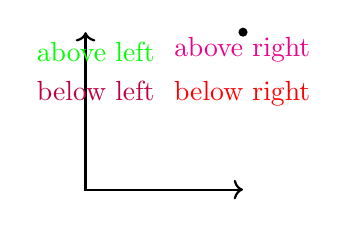
\begin{tikzpicture}[scale=2]
    \draw [thick, <->] (0,1) -- (0,0) -- (1,0);
    \draw[fill] (1,1) circle [radius=0.025];
    \node [below right, red] at (.5,.75) {below right};
    \node [above left, green] at (.5,.75) {above left};
    \node [below left, purple] at (.5,.75) {below left};
    \node [above right, magenta] at (.5,.75) {above right};
\end{tikzpicture}
\end{lstlisting}

\begin{center}
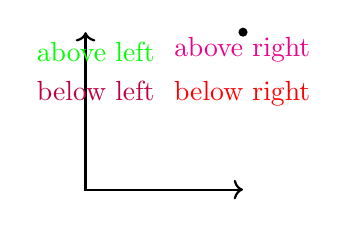
\begin{tikzpicture}[scale=2]
\draw [thick, <->] (0,1) -- (0,0) -- (1,0);
\draw[fill] (1,1) circle [radius=0.025];
\node [below right, red] at (.5,.75) {below right};
\node [above left, green] at (.5,.75) {above left};
\node [below left, purple] at (.5,.75) {below left};
\node [above right, magenta] at (.5,.75) {above right};
\end{tikzpicture}
\end{center}


\subsection{Algunos ejemplos adicionales}

\begin{lstlisting}[frame=single]
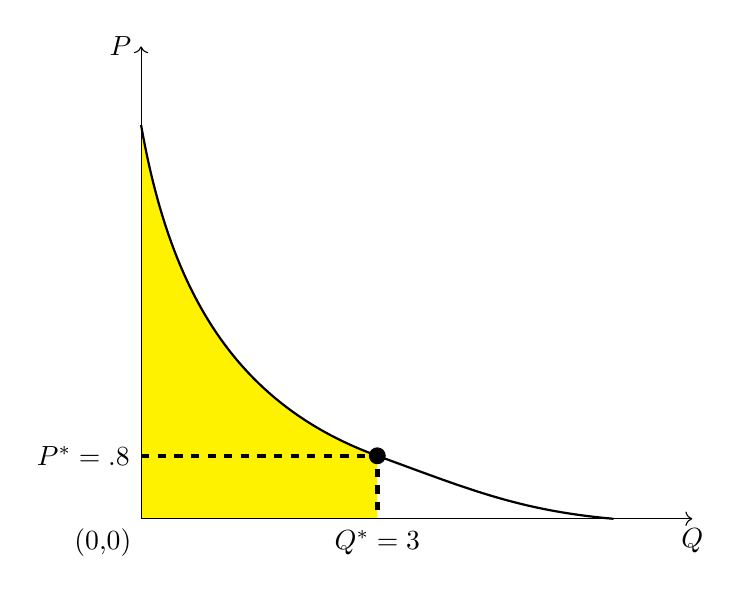
\begin{tikzpicture}
    \path [fill=yellow] (0,0) -- (0,5) to [out=-80, in=160]
    (3,.8) -- (3,0) -- (0,0);
    \draw [<->] (0,6) node [left] {$P$} -- (0,0)
    node [below left] {(0,0)} -- (7,0) node [below] {$Q$};
    \draw [ultra thick, dashed] (0,.8) node [left] {$P^*=.8$} -- (3,.8)
    -- (3,0) node [below] {$Q^*=3$};
    \draw [fill] (3,.8) circle [radius=.1];
    \draw [thick] (0,5) to [out=-80, in=160] (3,.8) to
    [out=-20, in=175] (6,0);
\end{tikzpicture}

\end{lstlisting}

\begin{center}
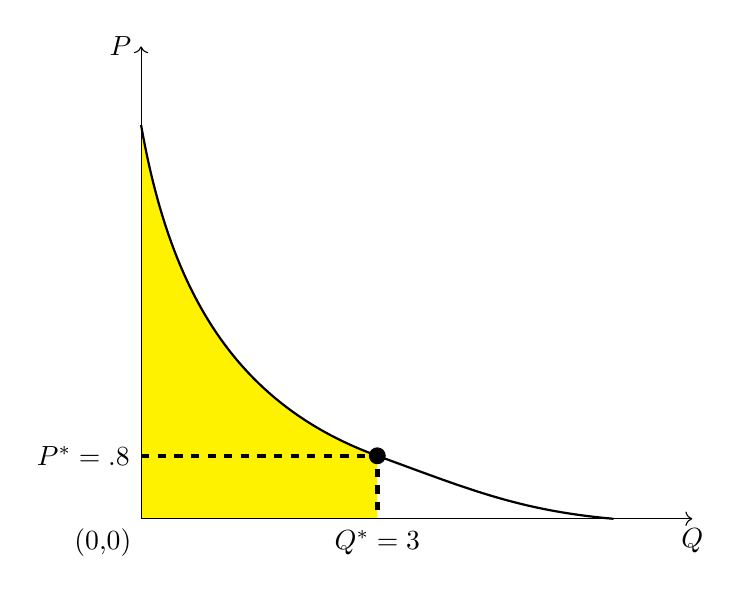
\begin{tikzpicture}
\path [fill=yellow] (0,0) -- (0,5) to [out=-80, in=160]
(3,.8) -- (3,0) -- (0,0);
\draw [<->] (0,6) node [left] {$P$} -- (0,0)
node [below left] {(0,0)} -- (7,0) node [below] {$Q$};
\draw [ultra thick, dashed] (0,.8) node [left] {$P^*=.8$} -- (3,.8)
-- (3,0) node [below] {$Q^*=3$};
\draw [fill] (3,.8) circle [radius=.1];
\draw [thick] (0,5) to [out=-80, in=160] (3,.8) to
[out=-20, in=175] (6,0);
\end{tikzpicture}

\end{center}

\begin{lstlisting}[frame=single]
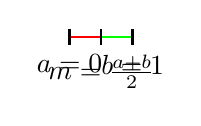
\begin{tikzpicture}[xscale=0.8] % Escalamiento 80%
    % Segmento de 0 a 1
    \draw[-][draw=red, thick] (0,0) -- (.5,0);
    \draw[-][draw=green, thick] (.5,0) -- (1,0);
    % Texto debajo ("below") del segmento
    \draw [thick] (0,-.1) node[below]{$a=0$} -- (0,0.1);
    \draw [thick] (0.5,-.1) node[below]{$m=\frac{a+b}{2}$} -- (0.5,0.1);
    \draw [thick] (1,-.1) node[below]{$b=1$} -- (1,0.1);
\end{tikzpicture}
\end{lstlisting}

\begin{center}
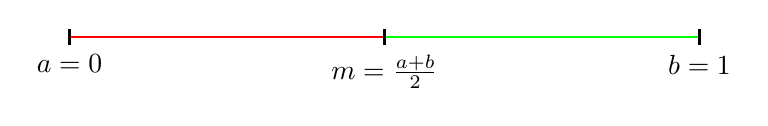
\begin{tikzpicture}[xscale=8] % Escalamiento 80%
% Segmento de 0 a 1
\draw[-][draw=red, thick] (0,0) -- (.5,0);
\draw[-][draw=green, thick] (.5,0) -- (1,0);
% Texto debajo ("below") del segmento
\draw [thick] (0,-.1) node[below]{$a=0$} -- (0,0.1);
\draw [thick] (0.5,-.1) node[below]{$m=\frac{a+b}{2}$} -- (0.5,0.1);
\draw [thick] (1,-.1) node[below]{$b=1$} -- (1,0.1);
\end{tikzpicture}
\end{center}

\begin{lstlisting}[frame=single]
\usetikzlibrary{matrix}
begin{tikzpicture}[scale=2]
    \matrix (m) [matrix of math nodes,row sep=3em,column sep=4em,minimum width=2em]
    {
     F_t(x) & F(x) \\
     A_t & A \\};
    \path[-stealth]
    (m-1-1) edge node [left] {$\mathcal{B}_X$} (m-2-1)
            edge [double] node [below] {$\mathcal{B}_t$} (m-1-2)
    (m-2-1.east|-m-2-2) edge node [below] {$\mathcal{B}_T$}
            node [above] {$\exists$} (m-2-2)
    (m-1-2) edge node [right] {$\mathcal{B}_T$} (m-2-2)
        edge [dashed,-] (m-2-1);
\end{tikzpicture}
\end{lstlisting}

\vspace{12pt}

\begin{center}
    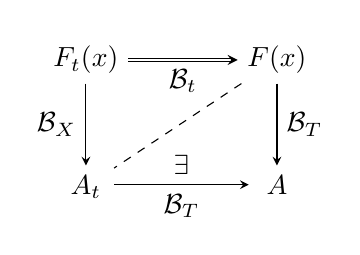
\begin{tikzpicture}[scale=2]
  \matrix (m) [matrix of math nodes,row sep=3em,column sep=4em,minimum width=2em]
  {
     F_t(x) & F(x) \\
     A_t & A \\};
  \path[-stealth]
    (m-1-1) edge node [left] {$\mathcal{B}_X$} (m-2-1)
            edge [double] node [below] {$\mathcal{B}_t$} (m-1-2)
    (m-2-1.east|-m-2-2) edge node [below] {$\mathcal{B}_T$}
            node [above] {$\exists$} (m-2-2)
    (m-1-2) edge node [right] {$\mathcal{B}_T$} (m-2-2)
            edge [dashed,-] (m-2-1);
\end{tikzpicture}
\end{center}

% \begin{lstlisting}[frame=single]
% \begin{tikzpicture}[line cap=round,line join=round,>=triangle 45]
%     \begin{axis}[
%     x=3.0cm,y=3.0cm,
%     axis lines=middle,
%     ymajorgrids=true,
%     xmajorgrids=true,
%     xmin=-0.1,
%     xmax=1.3,
%     ymin=-0.1,
%     ymax=1.3,
%     xtick={0,0.5,1},
%     ytick={0,0.5,1}]
%     \clip(-0.1,-0.1) rectangle (1.3,1.3);
%         \draw [line width=1.4 pt] (0.,0.)-- (0.5,1.);
%         \draw [line width=1.4 pt] (0.5,0.5)-- (1.,0.5);
%         \draw [fill=colordef] (1.,0.5) circle (2.5pt);
%         \draw [fill=colordef] (0.5,0.5) circle (2.5pt);
%         \draw [fill=white] (0.5,1.) circle (2.5pt);
%         \draw [fill=colordef] (0.,0.) circle (2.0pt);
%     \end{axis}
% \end{tikzpicture}
% \end{lstlisting}

% \begin{center}
%     \begin{tikzpicture}[line cap=round,line join=round,>=triangle 45]
%     \begin{axis}[
%     x=3.0cm,y=3.0cm,
%     axis lines=middle,
%     ymajorgrids=true,
%     xmajorgrids=true,
%     xmin=-0.1,
%     xmax=1.3,
%     ymin=-0.1,
%     ymax=1.3,
%     xtick={0,0.5,1},
%     ytick={0,0.5,1}]
%     \clip(-0.1,-0.1) rectangle (1.3,1.3);
%         \draw [line width=1.4 pt] (0.,0.)-- (0.5,1.);
%         \draw [line width=1.4 pt] (0.5,0.5)-- (1.,0.5);
%         \draw [fill=colordef] (1.,0.5) circle (2.5pt);
%         \draw [fill=colordef] (0.5,0.5) circle (2.5pt);
%         \draw [fill=white] (0.5,1.) circle (2.5pt);
%         \draw [fill=colordef] (0.,0.) circle (2.0pt);
%     \end{axis}
% \end{tikzpicture}
% \end{center}

Para los siguientes diagramas se requiere la librería \verb@cd@; así, debemos incluir:

\begin{lstlisting}[frame=single]
\usetikzlibrary{cd}
\end{lstlisting}

Además de la declaración de los signos \verb@"@ para evitar conflictos con el paquete \verb@babel@, esto se soluciona incluyendo el siguiente comando luego del \verb@\begin{document}@

\begin{lstlisting}[frame=single]
\shorthandoff{"}
\end{lstlisting}

Con ello, consideremos los siguientes ejemplos:

\begin{lstlisting}[frame=single]
\begin{tikzcd}
    A\arrow[rd] \arrow[r, "\phi"] & B \\
    & C
\end{tikzcd}
\end{lstlisting}

\begin{center}
\begin{tikzcd}
A\arrow[rd] \arrow[r, "\phi"] & B \\
& C
\end{tikzcd}
\end{center}

\begin{lstlisting}[frame=single]
\begin{tikzcd}
    T
    \arrow[drr, bend left, "x"]
    \arrow[ddr, bend right, "y"]
    \arrow[dr, dotted, "{(x,y)}" description] & & \\
    & X \times_Z Y\arrow[r, "p"]\arrow[d, "q"]
    & X\arrow[d, "f"] \\
    & Y\arrow[r, "g"]& Z
\end{tikzcd}
\end{lstlisting}

\begin{center}
\begin{tikzcd}
    T
    \arrow[drr, bend left, "x"]
    \arrow[ddr, bend right, "y"]
    \arrow[dr, dotted, "{(x,y)}" description] & & \\
    & X \times_Z Y\arrow[r, "p"]\arrow[d, "q"]
    & X\arrow[d, "f"] \\
    & Y\arrow[r, "g"]& Z
\end{tikzcd}
\end{center}

\subsection{Graficar datos}

Una de las formas más usuales de realizar gráficos es en base a un archivo de datos que proporciona los puntos a graficar. En este sentido, es posible graficar esos datos directamente en \LaTeX{}, para ello requerimos el paquete \verb@pgfplotstable@ y un archivo de texto plano (\verb@.txt@) con los datos separados por un espacio simple, con decimales separados por puntos y con un título en cada columna para poder especificar la columna de datos a tomar.  


Para ilustrar el funcionamiento de esta opción consideremos el siguiente caso: Para una exposición se requiere un gráfico que relacione las dimensiones de una matriz con su número de condición\footnote{En el campo del análisis numérico, el número de condición de una función respecto de su argumento mide cuánto se modifica el valor de salida si se realiza un gran cambio en el valor de entrada. (Wikipedia, 2021)}; para ello se han exportado los datos a un archivo con las características requeridas de nombre \verb@Datos.txt@ y con el siguiente contenido:

\begin{lstlisting}[frame=single]
num A Atil
0 0 0
0 0 0
0 0 0
4 3 2.08
9 9 4.77
16 13.33 7.3
25 20.77 11.07
36 27.45 14.77
49 37.26 19.56
64 46.3 24.43
81 58.48 30.34
100 69.86 36.41
121 84.41 43.5
144 98.15 50.76
169 115.06 59.04
196 131.15 67.5
225 150.42 76.97
256 168.87 86.64
289 190.49 97.3
324 211.3 108.16
361 235.29 120.01
400 258.45 132.07
441 284.79 145.12
484 310.32 158.38
529 339.01 172.62
576 366.9 187.07
625 397.95 202.51
\end{lstlisting}

Notemos que nuestro archivo posee 3 columnas con sus respectivos títulos. A continuación procedemos a realizar la gráfica respectiva, para ello consideremos el siguiente código:

\begin{lstlisting}[frame=single]
\begin{tikzpicture}[scale=0.75]
    \begin{axis}[
        xlabel={Dimensión de la matriz},
        ylabel={Número de condición},
        legend pos=north west,
        legend entries={Sin condicionar,Condicionada},
        ]
        \addplot table [x=num,y=A,color=colordef] {Datos.txt};
        \addplot table [x=num,y=Atil] {Datos.txt};
    \end{axis}
\end{tikzpicture}
\end{lstlisting}

y obtenemos el siguiente gráfico:

\begin{center}
\begin{tikzpicture}[scale=0.75]
\begin{axis}[
    xlabel={Dimensión de la matriz},
    ylabel={Número de condición},
    legend pos=north west,
    legend entries={Sin condicionar,Condicionada},
    ]
    \addplot table [x=num,y=A] {Datos.txt};
    \addplot table [x=num,y=Atil] {Datos.txt};
\end{axis}
\end{tikzpicture}
\end{center}

Notemos que de esta manera es posible optimizar el tiempo requerido para actualizar los gráficos en el caso de que los datos cambien. Más información sobre este paquete puede ser encontrada en: \href{https://ctan.org/pkg/pgfplotstable}{https://ctan.org/pkg/pgfplotstable}.

\end{document} 